\chapter{Método}

\graphicspath{ {/var/www/html/meninadasbalas/project/monografia/latex/images/} }

Neste capítulo descreveremos as tecnologias utilizadas para o desenvolvimento do projeto.

% =========================================================================== %
\section{Pré desenvolvimento}

\subsection{Hosting}
Como dito anteriormente, temos muitas opções de servidores para instalarmos este e-commerce. Para a escolha, foi levada em consideração a recomendação dos usuários do framework que será utilizado (será explanado na próxima seção) postado em \url{www.drupal.org/hosting}, o preço oferecido, a quantidade de domínios possíveis e o espaço em disco disponibilizado. As melhores opções na época de contatação do serviço eram:

\begin{table}[h]
  \begin{center}
    \begin{tabular}{ | l | r | r | r |}
      \hline
      Nome & Espaço & Domínios & Valor mensal\\ \hline
      Bluehost & Ilimitado & 3 & R\$ 15,90 \\ \hline
      Hostgator & Ilimitado & Ilimitado & R\$ 9,99 \\ \hline
      GoDaddy & Ilimidado & Ilimitado & R\$ 10,99 \\ \hline
      SiteGroud & 20 GB & Ilimitado & R\$ 14,99 \\ \hline
    \end{tabular}
    \caption{Opções de hosting para o e-commerce.}
    \label{hosting}
  \end{center}
\end{table}

Deste, foi escolhido o serviço da empresa Hostgator, por oferecer espaço e domínios ilimitados e o menor preço.

\subsection{Domínio}
Como também é um fator importante para SEO\footnote{Search engine optimization - uma forma de aumentar os acessos do seu site através de um conjunto de técnicas e estratégias que permitem que um site melhore seu posicionamento nos resultados orgânicos dos mecanismos de busca, como Google e Bing\cite{SEO}.}, foi sugerido ao cliente escolher um nome de domínio simples, fácil de ser associado com a marca e com um top level domain (TLD ou domínio de nível superior) que dê credibilidade ao site como por exemplo o `.com` ou `.com.br`. No caso deste último, a indexação será melhor em uma busca nacional \cite{TLD}. Foi então combinado de usar o nome da empresa com o TLD mais utilizado, com mais de 90\% dos sites brasileiros \cite{RegistroBr}, ficando como a seguir:

\begin{figure}
  \centering
    \large
    https://meninadasbalas.com.br
\end{figure}

Comprado online na empresa GoDaddy \url{br.godaddy.com}, foi pago R\$ 44,99 por 1 ano de direito de uso deste domínio.

% =========================================================================== %
\section{Drupal}

Como base para o o e-commerce utilizaremos o framework e gerenciador de conteúdo Drupal. Este software foi criado em 2000 pelo estudante universitário belga Dries Buytaert para ser um pequeno gerenciador de postagem um blog. Mais tarde em 2001, o código deste sistema foi aberto ao público, com o intuito de permitir as pessoas pudessem realizar experimentos e construir extenções. Desde então, o número de usuários vem crescendo a cada ano e sua comunidade de desenvolvedores melhorando o código diariamente. Hoje o Drupal conta com mais de 37 mil extenções \cite{DrupalModules}, chamadas de módulos, com diversas funcionalidades e utilizando as mais novas tecnologias, além de mais de 2 mil temas \cite{DrupalTheme}.

Os motivos desta escolha foram:

\begin{itemize}
  \item Segurança: Muitas camadas de proteção são oferecidas pelo Drupal, desde controle de acesso de usuários à API's que protegem o sistema de ataques.
  \item Flexibilidade: Podemos usá-lo para todo e qualquer tipo de site ou serviço online e seu sistema pode ser adaptado para qualquer projeto.
  \item Comunidade: A quantidade e qualidade das extenções providas pela comunidade para adicionar as mais diversas funcionalidades.
  \item Experiência: Prévia experiência com o framework, o que facilita o design e desenvolvimento do sistema e-commerce.
\end{itemize}

\subsection{Drupal 8}

A versão estável mais recente do Drupal é a número 8 e será a utilizada no projeto. Comparada com a versão anterior, temos um sistema de \textit{cache}\footnote{É um dispositivo de acesso rápido, interno a um sistema, que serve de intermediário entre um operador de um processo e o dispositivo de armazenamento ao qual esse operador acede\cite{Cache}.} muito mais potente, módulos importantes adicionados ao núcleo, a mudança do sistema de templates de PHP\footnote{Hypertext Preprocessor: Linguagem de script para servidores} para Twig\footnote{Linguagem para construção de templates HMTL.}, segurança reforçada e novas tecnologias e padrões sendo absorvidos. 

\subsection{Núcleo}

Ao instalar o Drupal nos deparamos com um site cru, mas com várias funciolidades já prontas para serem utilizadas. Algumas delas serão de suma importância para atingirmos nossos objetivos e serão listadas abaixo, pelo nome do módulo no núcleo.

\subsubsection{Node}
O gerênciamento de conteúdo é algo nativo do Drupal, então planejaremos quais os tipos que teremos no site. Cada conteúdo, conhecido como node, pode ter campos configuráveis, que podem representar propriedades do mesmo como por exemplo título, descrição, imagem, relação com outro conteúdo, autor, entre outros. Alguns deles como título, autor e status de publicação são padrões para todos.

Planejamos quatro tipos de conteúdo:
\begin{itemize}
  \item Banner - Representando o textit{banner} da página inicial, tendo campos para título, um subtítulo e uma imagem.
  \item Review - Representando as opiniões dos usuários sobre os produtos com um campo de texto e o título automático, para facilitar a criação deste conteúdo.
  \item Article - Postagens gerais de conteúdo aberto, com título, imagens e textos.
  \item Opinion - Representando os opiniões dos usuários sobre a empresa.
\end{itemize}

Poderiamos considerar o produto também um conteúdo, mas como veremos adiante, este é uma entidade a parte, criada por um módulo da comunidade.

\subsubsection{Taxonomy}
Já pensando nos produtos, criaremos um vocabulário de taxonomia\footnote{Taxonomia é a ciência de classificar itens.}, que é uma lista de keywords utilizadas para organizar o conteúdo do site. Estas \textit{keywords} serão os sabores de balas que a empresa fabrica e serão atrelados a cada produto, para facilitar a posterior filtragem e exibição destes.

\subsubsection{Views}
Modo mais comum de exibir grupos de conteúdo no Drupal, o módulo Views é um dos que na versão anterior não eram parte do núcleo do sistema e por sua importância foi incorporado. Ele permite filtragem e ordenação de conteúdo por valores de propriedades e a exibição dos item resultantes. 

Com ele, faremos os blocos de \textit{banners}, \textit{reviews}, notícias, produtos e opiniões da \textit{homepage}a.
\begin{itemize}
  \item Banner: Os 3 conteúdos do tipo \textit{banner} em formato de carrossel automático.
  \item Notícias: As 3 notícias mais recentes postadas.
  \item Reviews: Os 4 reviews mais visualizados.
  \item Opiniões: 3 opiniões escolhidas pelo administrador.
\end{itemize}

Além dos blocos, faremos também as páginas de listagem de produtos, reviews, opiniões e notícias.

\subsubsection{User}
Responsável pelo gerenciamento dos usuários do site e suas permissões, este módulo nos permitirá ter usuários logados com todas as informações necessárioas para o fluxo de compras e criação de conteúdo.

\subsubsection{Menu}
Este módulo, como o nome já diz, cria menus com ancoras para outros lugares do site ou sites externos. Segue a listagem dos menus do site, com nome, localização e função:

\begin{itemize}
  \item Topbar Contact Menu: Localizado no topo da página, terá apenas dois links para a página de contato.
  \item Topbar User Menu: Também no top da página, terá links de login e registro para usuários anônimos e links para detalhes da conta e sair para usuários logados.
  \item Main Menu: Menu principal, na parte superior do site com links para as páginas mais importantes.
  \item Footer Menu: No rodapé do site, menu com links para loja, página de contato e informações em geral.
\end{itemize}


% =========================================================================== %
\section{Ambiente de Desenvolvimento}

Com o framework escolhido, vamos construir o ambiente de desenvolvimento. 

\subsection{Sistema operacinal e máquina virtual} 
Utilizaremos o sistema operacional Ubuntu 16.04 e esporadicamente OSX El Capitan para desenvolvimento local e no servidor temos um CentOS 6. Para evitar problemas de compatibilidade como dito no capítulo de introdução, utilisaremos para desenvolvimento local uma máquina virtual (VM) com as mesmas configurações do servidor. O gerenciamento e configuração desta será feita por um software especializado chamado Vagrant.

Será usada uma configuração pré-definida criada por Jeff Geerling \url{www.drupalvm.com/}, Arquiteto Drupal, onde o Vagrant cria uma máquina virtual e a configura, com todos os programas e ferramentas que serão necessárias para o desenvolvimento neste framework. Alteramos somentes os pontos onde temos que imitar o servidor Hostgator, que é a versão dos softwares Apache2 e MySQL e a versão da linguagem PHP. Isso já nos garante o funcionamento estável e previsível do nosso site em todos os ambientes que ele estiver instalado.

\subsection{Apache, PHP e MySQL}
Apesar do Drupal funcionar com vários softwares de servidores web, como Nginx e Hiawatha, o mais utilizado é o Apache2. Além disso, nosso servidor no Hostgator também roda Apache2, na versão 2.2.25, então este é a escolha inevitável. 

Para a linguagem de servidor, o Drupal 8 requer PHP na versão mínima 5.5.9 e no servidor podemos escolher entre 5.5, 5.6 e 7.0. Foi escolhido a versão 7.0 por ser mais rápida \cite{PHP7Velocidade} e possuir funcionalidades mais avançadas e seguras que a versão 5.6 \cite{PHP7}.

O software de banco de dados será o MySQL versão 5.6.32, que é a única opção no servidor e foi verificada a versão utilizada.

\subsection{Fluxo}
O código será versionado pelo software Git e salvo em repositório público remoto mantido pela empresa Github \url{www.github.com}. Quando cada pequena tarefa for terminada, um commit é feito com uma breve descrição do que foi feito. Versões de teste serão carregadas para o servidor via SSH\footnote{É um protocolo de rede criptográfico para operação de serviços de rede de forma segura sobre uma rede insegura\cite{SSH}.}, também utilizando o Git. Um subdomínio será criado para esta versão de teste, adicionando `dev.` no endereço do site. Esta versão será exclusivamente para testes e deverá ter acesso restrito ao publico em geral. Assim que uma versão estável for atingida, mesmo que sem todos os requisitos do site alcançados, esta será carregada para o ambiente de produção, no domínio principal. O objetivo deste fluxo é ter o máximo de funcionalidades possives antes de inaugurar o site.

\subsection{Composer}
Iremos utilizar o software gerenciador de pacotes Composer para instalar o Drupal e suas dependências e posteriormente os módulos da comunidade que serão necessários. Uma boa base para o projeto pode ser o Drupal-Composer Project \url{www.github.com/drupal-composer/drupal-project}, código de configuração e scripts do Composer que montam o Drupal com a estrutura de arquivos requirida por ele.

A fork is a copy of a repository. Forking a repository allows you to freely experiment with changes without affecting the original project.

Porém, um problema foi detectado no uso deste pacote. O Drupal é instalado em um sub-diretório do projeto e não na raiz. Isso nos impede de utilizar o domínio principal quando o site for instalado no servidor, pois os arquivos tem que estar na raiz do diretório. Para resolver isto, criamos uma fork\footnote{É uma cópia do repositório que permite modificações e experimentos sem mundanças no repositório original.} \url{https://github.com/renanmfd/drupal-project} deste projeto no Github e modifiquei todos os códigos e configurações para instalar o Drupal no diretório raíz. Esta fork foi carregada no site Packagist \url{https://packagist.org} para ficar disponível para \textit{download} via Composer, com o comando:

\begin{lstlisting}
  composer create-project drupal-composer/drupal-project:8.x-dev 
    meninadasbalas --stability dev --no-interaction
\end{lstlisting}

Com o problema sanado, podemos dar incio ao processo de instalação do Drupal e logo após a fase de codificação do projeto.

% =========================================================================== %
\section{Front-end}

\subsection{Bootstrap}
Para o estilo ou tema do site, utilizaremos um dos melhores e mais utilizados frameworks de CSS e Javascript que existe atualmente, o Boostrap\cite{Bootstrap}. A escolha deste se deu simplesmente pelo conhecimento prévio e facilidade de uso. Com ferramentas para design responsivo e bibliotecas Javascript para funcionalidades que serão necessárias como por exemplo, o carrossel de \textit{banners}, este framework é a melhor opção para este projeto. No momento do desenvolvimento deste projeto a versão mais estável é a 3.

\subsection{Temas Drupal}
Na comunidade de Drupal, temos um tema Boostrap, que é uma base para sites que pretendem utilizar esta ferramenta para constriur seus layouts. Este é nosso primeiro requerimento do projeto, instalado via Composer.

\begin{lstlisting}
  \$ composer require drupal/bootstrap
\end{lstlisting}

Criaremos um sub-tema, com base no Bootstrap para Drupal que será chamado `MBC Theme`. Neste tema teremos os arquivos de CSS, imagens utilizadas pelo CSS, Javascript, templates Twig e um arquivo de PHP onde podemos modificar e adicionar as variáveis que são passadas os templates. 

Em seguida, para facilitar o desenvolvimento, vamos instalar também um tema administrativo, que como o adjetivo já diz, só é utilizado nas páginas administrativas do site. Foi escolhido o tema Adminimal Theme, por ser um dos temas desta categoria mais utilizados e proporcionar uma interface responsiva e limpa.

\begin{lstlisting}
  \$ composer require drupal/adminimal_theme
\end{lstlisting}

\subsection{LESS}
Less é um pré-processador de CSS que extende a linguagem, adicionando melhorias como variáveis, funções e várias outras técnicas que deixam a manutenção do CSS mais fácil \cite{Less}. Ela foi escolhida por ser utilizada nativamente no framework Bootstrap versão 3.

\begin{figure}[ht]
  \centering
  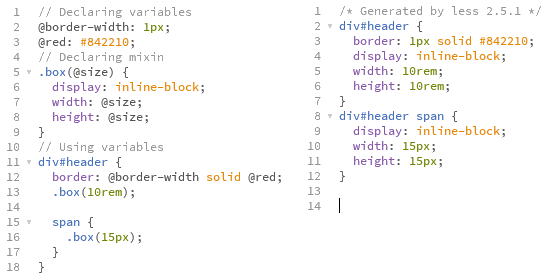
\includegraphics{lesstocss}
  \caption{Algumas funcionalidades do LESS em um código simples e seu resultado após compilado.}
  \label{lesstocss}
\end{figure}

O tema do site será desenvolvido da forma mais modular possível, cada bloco minimo do site tendo seu próprio arquivo, que serão unificados e processados pelo compilador do LESS. A intenção é facilitar a futura melhoria de performance, carregando na página apenas o estilo dos blocos que estão nela. Inicialmente, todos serão incluídos e transformados em um único arquivo de CSS que carregara em todas as páginas.

\subsection{Javascript}
Interações e efeitos mais avançados em páginas web são feitos pelo Javascript (JS), linguagem de script interpretada pelo browser, que tem acesso a toda a estrutura do site. O carrossel de baners na homepage irá utilizar uma das funcionalidades que o JS do framework Bootstrap disponibiliza.

Para garantir qualidade do código JS, utilizaremos a ferramenta ESLint criada por Nicholas C. Zakas em 2013. Esta analiza o código e avisa sobre estruturas que não seguem  padrões de código ou são consideradas inseguras.

\subsection{jQuery}
Para facilitar o desenvolvimento com Javascript e por ser um requerimento do Boostrap, utilizaremos a biblioteca jQuery. Esta possui várias funções que são muito utilizadas no desenvolvimento o que facilita algumas tarefas.

\begin{figure}[ht]
  \centering
  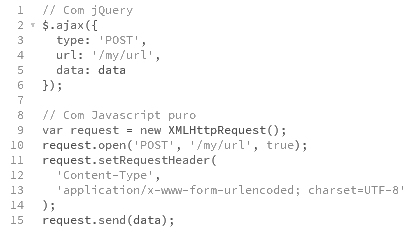
\includegraphics{jquery}
  \caption{Diferença entre Javascript puro e jQuery ao fazer um request HTTP do tipo POST.}
  \label{jquery}
\end{figure}

\subsection{NPM e Gulp}
Para fechar o ambiente de front-end, utilizaremos o automatizador de tarefas Gulp e alguns pacotes de extenção que ele possui. O Gulp e suas extenções são escritas em Javascript e executam em ambiente do NodeJS. Para instalá-los, utilizamos o gerenciador de pacotes do NodeJS chamado Node Package Manager (NPM). Após instalar o NodeJS e o NPM, utilizamos os seguintes comandos para instalar o Gulp e seus pacotes.

\begin{figure}[ht]
  \centering
  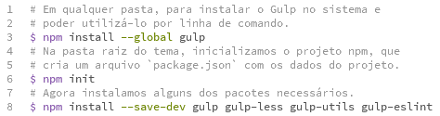
\includegraphics{npm_gulp}
  \caption{Comandos para instalação do Gulp em um terminal.}
  \label{npm_gulp}
\end{figure}

O Gulp é utilizado via código Javascript, onde utilizamos seus plugins para automatizar tarefas de front-end. As seguintes tarefas serão implementadas:

\begin{itemize}
  \item Less Hint - Ferramenta de análise de código LESS que ajuda na escrita limpa e consistente.
  \item Less Compile - Compila o arquivo principal do LESS, o qual importa todos os outros e gera um CSS minificado e com \textit{sourcemap}\footnote{Arquivo que acompanha minificação e mapeia para o \textit{browser} onde está cada elemento na origem não minificada, normalmente utilizada somente para desenvolvimento.}.
  \item JS Lint - Análise de código JS para evitar estruturas inseguras e garantir que os padrões de código sejam seguidos.
  \item JS Minification - Minificação dos arquivos de de Javascript para melhorar performance.
  \item Image Minification - Minificação do arquivos de imagens do tema também para performance.
  \item Favicon Creation - Criação de uma gama de arquivos de favicon, para que vários tipos de aplicativos, sistemas operacionais e programas tenham o favicon do tamanho correto, a partir de uma  única imagem.
  \item Watch - Escaneia todos os arquivos do tema para mudanças e executa as tarefas especificas ao arquivo que mudou. Por exemplo, a cada vez que um arquivo de LESS for salvo, o arquivo principal é compilado e um novo CSS estará disponível, já com as mudanças salvas.
\end{itemize}

No anéxo 1, temos a lista dos pacotes do NodeJS utlizados e o arquivo de configuração do Gulp.

% =========================================================================== %
\section{Commerce}
O Commerce é um modulo do Drupal para construção de lojas online que pode ser considerado como sendo um framework pelo tamanho e extensividade. Existem vários módulos que extendem o Commerce, adicionando funcionalidades, como por exemplo, diversos métodos de pagamento e serviços de entrega de produtos. Este módulo nos permite criar várias lojas, produtos, tipos de produtos e tipos de variantes de produtos.

\subsection{Produto}
Nosso site terá apenas uma loja. Uma loja extra é necessária quando por exemplo os produtos são enviados de lugares diferentes e produtos deste lugares não podem estar juntos em um pedido, o que não é o nosso caso.

Nosso único tipo de variante de produto será a bala de coco. Variantes são pequenas variações nas propriedade dos produtos podem ser representadas por campos. No caso deste trabalho, a utilização de variantes implicaria em termos somente duas páginas de produtos, a da bala tradicional e da bala recheada, com um formulário para a escolha das características, como se fosse por exemplo uma página de um computador na Amazon, com opções de tamanho de memória RAM. Neste conteúdo teremos campos gerais para as balas, como imagem, preço, descrição e sabor.

Para os tipos de produtos, teremos dois. Um representará a bala tradicional sem campos adicionais e outro a bala recheada com um campo de sabor de recheio. Esta propriedade esta relacionada as diferentes características que um produto pode ter e tem que estar relacionada com um tipo de variante, no nosso caso, a bala de coco.

O produto em si, será o conteúdo final a ser mostrado pela loja, deverá ser de um dos tipos de produto criados e pertencentes a uma ou mais lojas.

Todo este fluxo ajuda o módulo a organizar o e-commerce de modo que a loja seja flexível em relação aos produtos que serão vendidos. No caso deste e-commerce, utilizamos pouco desta flexibilidade por ter apenas dois tipos de produto.

\subsection{Cart}
O Commerce nos proporciona um carrinho de compras atrelado a conta do usuário. Todo produto pode ter um botão para adicioná-lo ao carrinho do usuário ativo. Se for um visitante, o carrinho é guardado do mesmo jeito, porém pelo id da sessão, fazendo deste um carrinho temporário. Tembém temos um bloco para a página inicial com um botão que abre um resumo dos itens selectionado pelo usuário e um link para a página de detalhes do carrinho.

\subsection{Shipping}
Para o sitema de serviço e pagamento da entregas, temos que utilizar uma integração com os correios. Esta integração não existe no Drupal 8, então será algo que iremos criar. Como este é uma parte complicada e deverá tomar um tempo, será utilizado um sitema de pagamento fixo por produto para a entrega, que é nativo do módulo Commerce Shipping e mais adinte, dedicaremos uma seção ao módulo de integração do Commerce, Drupal 8 e a API dos Correios do Brasil.

\subsection{Checkout}
O processo de compra também é gerenciado pelo Commerce. O carrinho, quando o usuário começa o fluxo de compra, é transformado em uma order. O fluxo acontece em 5 etapas:

\begin{itemize}
  \item Identificação: O usuário que não estiver logado, será pedido que entre com seu e-mail e senha ou que registre para uma nova conta no site.
  \item Informações: Nesta etapa será pedido ao usuário informações de contato, dados para envio, tipos e valores de envios e tipo de pagamento a ser utilizado.
  \item Revisão: Todos os dados da compra são exibidos para o usuário conferir os dados.
  \item Pagamento: Será requisitado os dados de pagamento ou haverá um redirecionamento para serviço de pagamento externo.
  \item Completo: Uma mensagem será exibida com o status do pedido e outras informações pertinentes.
\end{itemize}

\subsection{Paypal}
Por ser o método de pagamento mais utilizado mundialmente\cite{PaymentMethods}, o Paypal tem uma integração bem consolidada no Drupal 8 e o módulo Commerce. Por estas razões, ele será a única forma de pagamento para o site inicialmente. Idealmente, gostariamos que o pagamento pudesser ser feito por serviços brasileiros como PagSeguro e MercadoPago, mas a integração destes com o Commerce ainda não existe ou está em desenvolvimento para o Drupal 8.

Para utilizar os serviços do Paypal, instalamos o módulo Commerce Paypal no nosso site, criamos uma conta no site do serviço e requerimos uma chave para sua API. Esta chave é utilizada pelo módulo Commerce para realizar o pagamento dos produtos sem sair do nosso sistema.

% =========================================================================== %
\section{Extendendo o Drupal}

Para continuar a construção das funcionalidades de back-end do site, temos que adicionar outros módulos da comunidade Drupal, além do Commerce. Listaremos os mais importantes:

\begin{itemize}
  \item Paragraphs - Prove mais flexibilidade no posicionamento dos elementos na criação de conteúdos.
  \item Shield - Adiciona um login e senha HTTP para bloquear acesso ao site, inclusive de mecanismos de busca.
  \item Social Login - Permite que usuarios se registrem no site por redes sociais.
  \item Display Suite - Melhora o gerenciamento dos modos de visualização dos conteúdos.
  \item Pathauto - Cria automaticamente \textit{aliases}\footnote{Endereços alternativos, normalmente mais semânticos que os originais.} para várias páginas do site de acordo com um padrão escolhido pelo administrador.
  \item Menu Block - Cria blocos de menus para serem utilizados em várias regiões do site.
\end{itemize}

No anexo \ref{appendix:Módulos} temos uma lista de todos os módulos Drupal instalados com uma descrição das suas funcionalidades.

% =========================================================================== %
\section{Performance}

Para termos um site rápido, que retém os clientes do negócio, utilizaremos algumas técnicas e descreveremos algumas que o Drupal 8 já utiliza como padrão.

\subsection{Minificação, Agregação e Compactação}
As mais simples das melhorias que afetam positivamente a performance de um website são a minificação, agregação e a compactação dos recursos que o browser tem que baixar para montar a página. 

A minificação é o processo de remover caractéres desnecessários dos arquivos, normalmente espaços e quebras de linhas e no caso do Javascript, renomeando funções e variáveis com nomes de um só caractere, sem mudar a lógica do script. Após a minificação, os arquivos minificados ainda podem ser utilizados pelo browser normalmente. O benefício é a diminuição do tamanho dos recursos do website.

A agregação é o processo de juntar todos os arquivos com mesma extenção no menor número possível de arquivos. Por exemplo, todos os recursos de CSS de um site, que no caso do Drupal 8 pode chegar a ser entre 30 e 50, são agregados e transformados em 3 arquivos maiores. Isso melhora a performance porque diminui o número de requisições o browser tem que fazer para montar a página.

A compactação é um processo que diminui o tamanho do arquivo com técnicas mais avançadas e requerindo que o browser faça a descompactação antes de utilizar os recursos. É a mesma situação de compactar um arquivo PDF na extenção ZIP, ele diminui o tamanho do arquivo, porém para utilizá-lo novamente temos que descompactar. Esta compactação é feita pelo servidor somente quando ele está habilitado a fazê-lo e a requisição possui  um header específico, que avisa a ele que o cliente está apto a receber recursos compactados.

O Drupal 8, em suas configurações, já habilita a compactação dos arquivos pelo servidor. Estas estão no arquivo .htaccess na raíz do projeto.

Apesar do Drupal ter uma funcionalidade de compactação de CSS e JS, vamos instalar um módulo da comunidade que o faz com ferramentas melhores e possui mais opções, entre elas a agregação de arquivos. Este módulo se chama Advanced Aggregation.

\subsection{Imagens}
Outro recurso que precisa ser minificado são as imagens do site e para isto utilizaremos o módulo TinyPNG.

Este módulo foi desenvolvido originalmente para o Drupal 7, sem versões para o Drupal 8. Por ser um módulo relativamente simples, fizemos a migração e adaptação deste módulo para o Drupal 8. Algumas características não foram implementadas por uma questão de tempo e simplicidade. Este módulo utiliza o serviço do site TinyPNG \url(www.tinypng.com) e sua API para minificar todas as imagens que são carregas no site. O código é bem breve, sendo somente uma função.

\begin{figure}[ht]
  \centering
  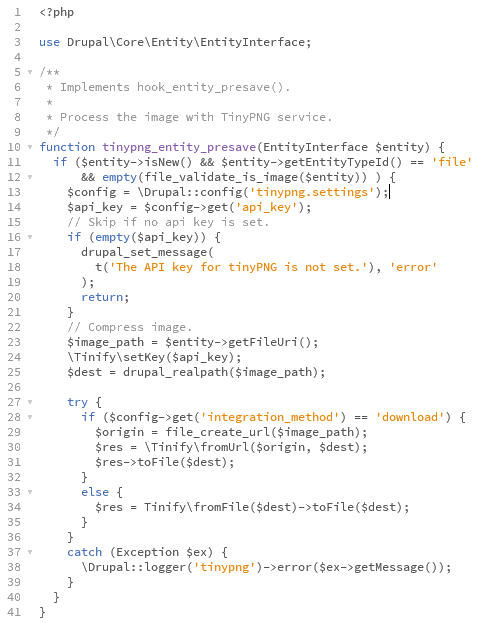
\includegraphics{tinypng_module}
  \caption{Código principal do módulo tinypng.}
  \label{tinypng_module}
\end{figure}

\subsection{Blazy}
Mais uma técnica utilizada é o \textit{Lazy Load}. Esta consiste em adiar o carregamento das imagens de uma página até que ela seja necessária. Se a imagem esta em uma parte visível da página, ela é carregada logo após a renderização do site e não durante. Isso reduz o tempo de carregamento de uma página por que diminui os recursos a serem baixados durante a renderização da página.

Para implementar esta funcionalidade utilizaremos o módulo Blazy do Drupal. Este adiciona formatadores de imagem que trocam o nome do atributo src para data-src da \textit{tag} HTML \emph{img}. Isso faz com que o \textit{browser} não baixe a imagem durante a renderização, por não ter uma atributo src. Após a renderização da página, um código Javascript troca o nome de volta para \textit{src}, fazendo com que o \textit{browser} identifique e baixe as imagens necessárias. As que estão em porções não visíveis da tela, este atributo será mudado de nome somente quando esta porção estiver visível.

\subsection{Técnicas}
Uma técnica imprescindível para melhorar a velociadade de um site é fazer com que partes dele que sejam estáticas sejam processadas pelo servidor somente uma vez e seu resultado salvo para ser utilizado em outras requisições. Isso se chama cache. O Drupal 8 possui um sistema bastante robusto de cache, que pode ser configurado para qualquer site. No nosso caso, utilizaremos as configurações que já vem padrão, somente desabilitando este cache nos ambientes de desenvolvimento.

\subsection{Medição}
A principal ferramenta que iremos utilizar para medir a performance do site é o serviço de análise GTMetrix do site \url{www.gtmetrix.com}. Esta ferramenta da notas a performance do site, baseadas em velocidade, boas práticas, quantidade de requests e tamanho total da página. Nos resultados, podemos ver dicas para melhorar a performance, mostrando o que foi feito e o que pode ser feito. Temos como objetivo conseguir no A (máxima) nas duas notas, PageSpeed e YSlow. Tentaremos implementar o máximo possível das dicas que forem dadas e as que não forem feitas, explicaremos o porque.

Como alternativa, usaremos também o serviço do Google chamado PageSpeed Insights, que com menos funcionalidades, faz esta mesma análise de boas práticas.


% =========================================================================== %
\section{Segurança}

Utilizando um framework sólido e em constante melhora foi a principal decisão quando pensamos na segurança do e-commerce. O Drupal e o módulo Commerce cuidam de praticamente tudo para que possamos entregar um website seguro para os clientes.

\subsection{Cuidados}
Apesar disto, algumas precauções devem ser tomadas:

\begin{itemize}
  \item Evitar lógicas complicadas em templates TWIG e filtrar conteúdo vindo do usuário antes de mostrar na tela, para evitar \textit{Cross Site Scripting}\footnote{Cross-site scripting (XSS) é um tipo de vulnerabilidade do sistema de segurança de um computador, encontrado normalmente em aplicações web que ativam ataques maliciosos ao injectarem client-side script dentro das páginas web vistas por outros usuários\cite{XSS}.}.
  \item Utilizar as camadas de abstração de banco de dados para evitar ataques de \textit{SQL Injection}\footnote{A Injeção de SQL, mais conhecida através do termo americano SQL Injection, é um tipo de ameaça de segurança que se aproveita de falhas em sistemas que interagem com bases de dados via SQL\cite{SQLInjection}.}.
  \item Garantir que as configurações do servidor e do site são as recomendadas pela comunidade Drupal, em \url{www.drupal.org/security/secure-configuration}.
\end{itemize}

\subsection{Certificado}
Para garantir que os dados de compras do usuário e do site fiquem seguros, é de extrema importância e uma necessidade tratando-se de um e-commerce, que tenhamos uma conexão encriptada. Para tal, temos que utilizar o protocolo de transferência HTTPS\footnote{Hyper Text Transfer Protocol Secure - protocolo de transferência de hipertexto seguro é uma implementação do protocolo HTTP sobre uma camada adicional de segurança que utiliza o protocolo SSL/TLS. Essa camada adicional permite que os dados sejam transmitidos por meio de uma conexão criptografada e que se verifique a autenticidade do servidor e do cliente por meio de certificados digitais.} em detrimento do mais comum HTTP\footnote{Hypertext Transfer Protocol, em português Protocolo de Transferência de Hipertexto, é um protocolo de comunicação utilizado para sistemas de informação na web\cite{HTTP}.} e comprar um certificado SSL\footnote{O protocolo SSL provê a privacidade e a integridade de dados entre duas aplicações que comuniquem pela internet\cite{SSL}.} para autenticação. Pagamos pelo certificado com 1 ano de validade o valor de R\$ 13,00 e mais um taxa de instalação no servidor para o HostGator de R\$ 60,00.

Para completar, no servidor, colocaremos um código de configuração para quando um acesso ao site acontecer pelo protocolo HTTP, ele seja redirecionado para o HTTPS, garantindo a segurança em todos os casos.
Além de ser um fator importante na segurança dos dados de um site, um certificado SSL é um fator levado em conta pelos mecanismos de busca.

% =========================================================================== %
\section{SEO}

\subsection{Metatags}
\textit{Metatags} são elementos do códgio HTML que representam dados que não são mostrados na tela. Estes são utilizados por serviços externos, como motores de buscas e redes sociais para obter informações sobre o site sem ter que escanear o seu conteúdo. Informações como autor, titulo, descrição, \textit{keywords}, imagem, linguagem, entre outras, são adicionadas via \textit{metatag}, como na imagem\ref{metatag} abaixo.

\begin{figure}[ht]
  \centering
  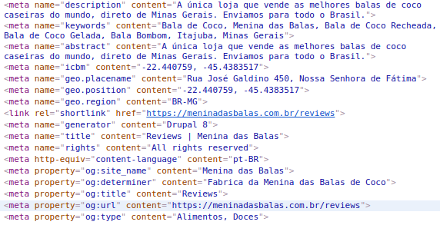
\includegraphics{metatag}
  \caption{Metatags do site no inspetor do Google Chrome.}
  \label{metatag}
\end{figure}

As \textit{metatags} acima\ref{metatag} com o atributo \textit{property} iniciando com \emph{og} são exemplos do protocolo Open Graph \url{http://ogp.me/}. Este protocolo criado pelo Facebook permite serviços externos terem informações sobre uma página da web de forma simples e que pode ser implementado facilmente pelo desenvolvedor. Quando formos compartilhar o link do site no Facebook ou outros serviços, ele escaneará a URL em busca destas \textit{tags} para montar um bloco com as informações, melhorando a visibilidade da empresa nesta rede social ou ferramenta. Outros sites, serviços e ferramentas também utilizam este protocolo.

Instalaremos o módulo Metatags do Drupal 8. Ele cria um conjunto de páginas administrativas  que permitem adicionar metatags de diversos protocolos em cada seção do site e também que estes sejam cadastrados via token, um \textit{placeholder} que diz qual informação a \textit{metatag} terá, baseado na página. Este token é um funcionalidade de outro módulo, requerido pelo Metatags, o Token. Ele nos permite, por exemplo, na configuração da metatag de título da página, colocar o token \textit{[current-page:url]}, que é troca pela URL da página quando esta for renderizada pelo back-end. Desta maneira, não precisamos configurar este campo para todas as páginas do site.

\subsection{Sitemap}
Para melhor indexação das nossas páginas nos mecanismos de busca, podemos criar e enviar um arquivo XML com os caminhos das páginas que podem ser indexados no site. O módulo do Drupal 8 Simple Sitemap toma conta desta tarefa, criando um XML ficará disponível no caminho \url{https://meninadasbalas.com.br/sitemap.xml} e será possível cadastra-lo nos motores de busca.

\subsection{Microdata}
\textit{Microdata}, assim como as \textit{metatags}, é utilizado para permitir que scripts externos reconheçam facilmente um página da web e saiba o que é cada elemento, sem ter que interpretar ou adivinhar. Este tipo de técnica é consiste em adicionar propriedades com valores específicos em \textit{tags} HTML. Estes valores indicam qual tipo de item o conteúdo deste HTML pertence. Para exemplificar, podemos utlizar para descrever um artigo, identificando onde está no HTML o título, corpo, imagem, autor e data de publicação.

\begin{figure}[ht]
  \centering
  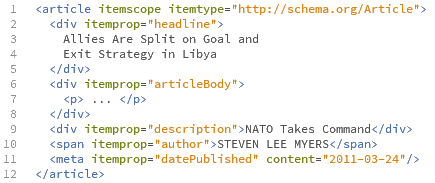
\includegraphics{microdata}
  \caption{Exemplo de utilização da técnica microdata no protocolo Schema.org.}
  \label{microdata}
\end{figure}

Por prover um melhor contexto para os motores de busca identificarem os conteúdos de uma página, esta técnica melhora muito a indexação de um site, além de melhorar a como os conteúdos do site aparecem no resultado da busca\cite{Microdata}.

No nosso site, utilizaremos \textit{microdata} em notícias, reviews, opiniões e produtos.

\subsection{Redes sociais}
Integração com redes sociais é quase um requerimento para websites de sucesso. Dar ao usuário um meio para facilmente compartilhar seu conteúdo no Facebook por exemplo, pode aumentar muito o número de visitas no site, além de ser vista com bom olhos pelos mecanismos de busca.

\subsection{Google Search Console}
Por fim, cadastraremos o nosso e-commerce na ferramenta Search Console do Google. Esta nos permite ter um visão de como está a indexação do site, quais os termos que quandos buscados o site aparece melhor colocado, quais modificações podem ser feitas para melhorar o a posição das páginas na busca, quais página do site tem erros, entre outras. Ela se mostra extremamente importante para o acompanhamento de campanhas de marketing e de análise do SEO de forma geral.
